% @author Arian Helberg

\chapter{Einleitung}
Effizientes Objektdesign und -modellierung sind entscheidende Kernfunktionalitäten in verschiedenen Bereichen der
digitalen Welt.
Da die Erstellung geometrischer Objekte für Laien unintuitiv ist und ein großes Maß an Erfahrung und Expertise
erfordert, ist dieses stetig komplexer werdende Feld für Neueinsteiger nur sehr schwer zu erschließen.
Die Forschung liefert hierzu einige Arbeiten zur prozeduralen Modellierung, um digitale Inhalte schneller
und automatisiert zu erstellen.
Gerade wenn es um die Darstellung natürlicher Umgebung geht, ist die Erstellung von ähnlichen Objekten, wie
zum Beispiel verschiedene Bäume derselben Gattung eines Waldes, ein schwieriges Problem.
Kleine Änderungen in prozeduralen Systemen können zu großen Veränderungen der Ergebnisse führen.
Darum beschäftigt sich die inverse prozedurale Modellierung unter anderem mit dem Inferieren von Regeln
und Mustern aus gegebenen Objekten, um diese nach bestimmten Regeln zu modellieren.
Ein wichtiges Werkzeug hierbei ist die Verwendung formaler Grammatiken als fundamentale Datenstruktur
der Informatik, um Strukturen zu beschreiben.
Eine spezielle Untergruppe sind die L-Systeme, die häufig bei der Beschreibung
von Verzweigungsstrukturen und Selbstähnlichkeit zum Einsatz kommen.
\\~\\
Diese Arbeit beschäftigt sich mit der Erstellung eines prozeduralen Systems zur Synthese von Ähnlichkeitsabbildern.
Hierzu soll über eine Benutzerschnittstelle eine Struktur erzeugt werden, aus der ein parametrisiertes L-Systems
inferiert werden kann, welches dann zur Generierung von ähnlichen Strukturen genutzt werden kann.

\newpage

\section{Problemstellung}
Während Methodiken zur Kodifizierung bestimmter Strukturen in den Bereich der prozeduralen Modellierung fällt,
findet das Ableiten von Regeln Anwendung in der inversen prozeduralen Modellierung.
Mit dem digitalen und naturwissenschaftlichen Fortschritt steigt die Anwendung immer komplexerer Strukturen, die
ein Herausarbeiten der schwer zu kontrollierenden, prozeduralen Regeln immer schwieriger machen.
\\~\\
Ein Beispiel hierzu aus der Gaming-Industrie ist die frühere Verwendung unorganisierter Modelle (ugs. Dreieckssuppe).
Diese Modelle weisen keine hierarchische Struktur auf und werden erst durch Datenstrukturen, wie bspw. Octrees organisiert.
Unorganisierte Modelle sind nur bedingt wiederverwendbar, da nur die vorliegende Modellierung genutzt werden kann.
Es besteht eine hohe Speicherkomplexität bei geringer Laufzeitkomplexität.
Für kleinste Veränderungen am Modell ist eine erneute Modellierung erforderlich, die wiederum Speicher benötigt, um sie
persistent speichern zu können.
Heutzutage werden die Objekte nach bestimmten Kriterien organisiert, um eine automatisierte Modellierung durch Algorithmen
zu ermöglichen, und so aus einer Grundstruktur weitere Modelle zu erzeugen.
Speicher- und Laufzeitkomplexität nähern sich an.
Aus diesem Grund werden allgemeingültige, vielseitig anwendbare Algorithmen gesucht, die bestimmte natürliche Eigenschaften
von Strukturen herausarbeiten (Reverse Engineering), um diese für die (inverse) prozedurale Modellierung zur
Verfügung zu stellen.
\\~\\
Diese Arbeit soll zeigen, wie sich durch die Erstellung eines Systems zur Generierung von ähnlichen Strukturen aus einer
Basistruktur, aktuelle Ansätze aus der Forschung in einem Programm umsetzen lassen.

\newpage

\section{Ziele}
Die Erstellung eines Systems zur Synthese von ähnlichen Strukturen aus einer Basis-struktur soll zentrale Aufgabe dieser
Arbeit sein.
Zunächst wird ein System benötigt, das eine Verzweigungsstruktur bestimmt, aus der die ählichen Strukturen erzeugt
werden können.
Um bestimmte Methodiken und Algorithmen der aktuellen Forschung auf die Eingabestruktur anwenden zu können, sollte diese
in einer Datenstruktur organisiert werden.
Anschließend kann ein L-System aus der Struktur inferiert werden.
Die inferierte Grammatik kann durch diverse Algorithmen verändert werden, bis das erzeugte L-System in der Lage ist
Ähnlichkeitsstrukturen zu bilden.

\section{Methodik}
Der Benutzer des Systems legt atomare Strukturen in Form von Zeichenketten an, die vom Programm eingelesen und
als Templates zur Verfügung gestellt werden.
Die Templates sind beliebig und können eine einfache Linie oder eine komplexe Verzweigung darstellen.
Werden diese Strukturen auf der graphischen Oberfläche platziert und mit diversen Transformationen verändert, spricht man
von Instanzen oder Template-Instanzen.

\subsection*{Strukturieren}
Der Benutzer verwendet die grafische Schnittstelle, um aus einzelnen Templates eine zusammenhängende Basisstruktur zu
erstellen.
Neben der Position der Instanzen werden Transformationsparameter, wie Rotation oder Skalierung, angepasst.

\subsection*{Visualisieren}
Der aktuelle Stand der Strukturierung ist jederzeit sichtbar.
Liniensegmente und Bindungselemente werden in einem graphischen Element visualisiert und für eine Interaktion zur Verfügung
gestellt.

\subsection*{Datenaufbereitung}
Das Ergebnis der Strukturierung wird in einer Baumstruktur
organisiert, in der jeder Knoten einer bestimmten Template-Instanz entspricht und die eingehende Kante die
geometrischen Transformationen relativ zum Elternknoten beschreibt.

\subsection*{Inferieren}
Aus der Baumstruktur kann eine formale Grammatik in Form eines L-Systems abgeleitet werden.
Diese Grammatik beschreibt lediglich die erstellte Basisstruktur und beinhaltet keine Transformationsparameter, da hier
nur auf die Topologie des Baumes und nicht auf geometrische Unterschiede der Instanzen eingegangen wird.

\subsection*{Komprimieren}
Um sich wiederholende Produktionsregeln zu vermeiden und so sowohl das Alphabet, als auch die Produktionsregelmenge
zu komprimieren, wird die Baumstruktur nach identischen, maximalen Unterbäumen durchsucht und durch zusammengefasste
Instanzen vereinfacht.
Hierbei gilt die Baumstruktur selbst nicht als Unterbaum.

\subsection*{Generalisieren}
Ähnliche Produktionsregeln des L-Systems werden mithilfe einer Kostenfunktion zusammengefasst, um diese mit
nicht-deterministischen Regeln zu generalisieren.
Die Kostenfunktion entscheidet hierbei über den Grad der Ähnlichkeit zweier Produktionsregeln.

\subsection*{Randomisieren}
Jedes Symbol der Grammatik nimmt eine Liste an Parametern entgegen, die nach bestimmten Kriterien pseudo-randomisiert
werden, um Variationen von Template-Instanzen zu erstellen.
Das Ausführen des L-Systems kann nun Ähnlichkeitsstrukturen für die Basisstruktur erzeugen.

\section{Aufbau}
Die Methodik zum Umsetzen des beschriebenen Systems wird wie folgt umgesetzt.

\begin{figure}[H]
    \centering
    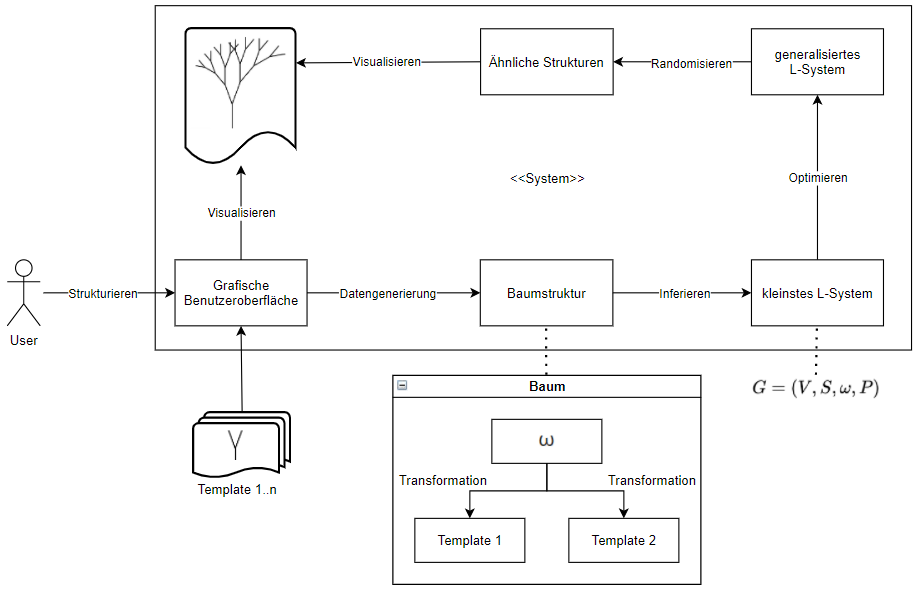
\includegraphics[width=14cm]{../images/System.PNG}
    \caption[Systemarchitektur]{Architektur des Systems mit einigen Datenstrukturen}
\end{figure}

Die Darstellung zeigt eine grobe Übersicht der Anwendungsfälle innerhalb des Systems.
Der Benutzer strukturiert vom System importierte Templates zu einer Basisstruktur mittels grafischer Bedienelemente.
Die Template-Instanzen werden hierbei in einer Baumtopologie organisiert.
Anschließend wird ein L-System aus der Baumstruktur generiert und komprimiert.
Das kompakte L-System wird generalisiert und ausgeführt.
Zuletzt wird das abgeleitete Axiom parametrisiert und sichtbar gemacht.